\documentclass[twoside]{article}
\usepackage{aistats2016}

\usepackage{xr}
\externaldocument[main-]{RejS-8}

%=============================================================================
% PACKAGES
%=============================================================================

\usepackage{url}
\usepackage{amsmath}
\usepackage{amssymb}
\usepackage{amsthm}
\usepackage{amsfonts}
\usepackage{braket}
\usepackage{complexity}
\usepackage{graphicx}% Include figure files
\usepackage{dcolumn}% Align table columns on decimal point
\usepackage{bm}% bold math
\usepackage{hyperref}
\usepackage{enumerate}
\usepackage{algorithm}
\usepackage{algpseudocode}
    \renewcommand{\algorithmicrequire}{\textbf{Input:}}
    \renewcommand{\algorithmicensure}{\textbf{Output:}}
    \newcommand{\inlinecomment}[1]{\Comment {\footnotesize #1} \normalsize}
    \newcommand{\linecomment}[1]{\State \(\triangleright\) {\footnotesize #1} \normalsize}
    %\renewcommand{\algorithmiccomment}[1]{\State\(\triangleright\) #1}
    
\usepackage{multirow}

%=============================================================================
% ENVIRONMENTS
%=============================================================================

\newtheorem{theorem}{Theorem}
\newtheorem{lemma}{Lemma}
\newtheorem{definition}{Definition}
\newtheorem{corollary}{Corollary}

\newenvironment{proofof}[1]{\begin{trivlist}\item[]{\flushleft\it
Proof of~#1.}}
{\qed\end{trivlist}}

%=============================================================================
% HYPERREF SETUP
%=============================================================================

\newcommand{\eq}[1]{\hyperref[eq:#1]{(\ref*{eq:#1})}}
\newcommand{\maineq}[1]{(\ref*{main-eq:#1}, main body)}
\renewcommand{\sec}[1]{\hyperref[sec:#1]{Section~\ref*{sec:#1}}}
\newcommand{\app}[1]{\hyperref[app:#1]{Appendix~\ref*{app:#1}}}
\newcommand{\fig}[1]{\hyperref[fig:#1]{Figure~\ref*{fig:#1}}}
\newcommand{\thm}[1]{Theorem~\ref*{main-thm:#1}}
\newcommand{\lem}[1]{Lemma~\ref*{main-lem:#1}}
\newcommand{\tab}[1]{\hyperref[tab:#1]{Table~\ref*{tab:#1}}}
\newcommand{\cor}[1]{Corollary~\ref*{main-cor:#1}}
\newcommand{\alg}[1]{\hyperref[alg:#1]{Algorithm~\ref*{alg:#1}}}
\newcommand{\defn}[1]{\hyperref[def:#1]{Definition~\ref*{def:#1}}}

%=============================================================================
% COMMANDS
%=============================================================================

\newcommand{\ketbra}[2]{|#1\rangle\!\langle#2|}
\newcommand{\prob}[1]{{\rm Pr}\left(#1 \right)}
% \newcommand{\Tr}[1]{{\rm Tr}\!\left[#1 \right]}
\newcommand{\expect}[2]{{\mathbb{E}_{#2}}\!\left\{#1 \right\}}
\newcommand{\var}[2]{{\mathbb{V}_{#2}}\!\left\{#1 \right\}}
\newcommand{\CRej}{\text{rejection filtering}}
\newcommand{\CSMC}{\text{SMC}}

\newcommand{\ess}{\mathrm{ess}}

\newcommand{\sinc}{\operatorname{sinc}}

% fix: supported only for revtex
%\newcommand{\openone}{\mathbb{I}}
% fix: unsupported with iopart
%\newcommand{\eqref}[1]{(\ref{#1})}

\newcommand{\sde}{\mathrm{sde}}
\newcommand{\Z}{\mathbb{Z}}
\newcommand{\RR}{\mathbb{R}}
\newcommand{\NN}{\mathrm{N}}
\newcommand{\w}{\omega}
\newcommand{\Kap}{\kappa}

\newcommand{\Tchar}{$T$}
\newcommand{\T}{\Tchar~}
\newcommand{\TT}{\mathrm{T}}
\newcommand{\ClT}{\{{\rm Clifford}, \Tchar\}~}
\newcommand{\Tcount}{\Tchar--count~}
\newcommand{\Tcountper}{\Tchar--count}
\newcommand{\Tcounts}{\Tchar--counts~}
\newcommand{\Tdepth}{\Tchar--depth~}
\newcommand{\Zr}{\Z[i,1/\sqrt{2}]}
\newcommand{\ve}{\varepsilon}
\newcommand{\defeq}{\mathrel{:=}}

\newcommand{\cu}[1]{{\textcolor{red}{#1}}}
\newcommand{\tout}[1]{{}}
\newcommand{\good}{{\rm good}}
\newcommand{\bad}{{\rm bad}}
\newcommand{\dd}{\mathrm{d}}

\newcommand{\id}{\openone}


\begin{document} %%%%%%%%%%%%%%%%%%%%%%%%%%%%%%%%%%%%%%%%%%%%%%%%%%%%%%%%%%%%%

%=============================================================================
% FRONT MATTER
%=============================================================================

\newcommand{\thetitle}{Bayesian inference via rejection filtering:\\ Supplemental Material }
% \twocolumn[
\onecolumn
  \aistatstitle{\thetitle}
  % \aistatsauthor{
  %   Nathan Wiebe$^\dagger$ \And
  %   Christopher Granade$^*$ \And
  %   Ashish Kapoor$^\ddagger$ \And
  %   Krysta M Svore$^\dagger$
  % }
  % \aistatsaddress{
  %   $^\dagger$QuArC \\ Microsoft Research \And
  %   $^*$EQuS \\ University of Sydney \And
  %   $^\ddagger$ASIG \\ Microsoft Research
  % }
% ]

\appendix

%=============================================================================
\section{Proofs of Theorems}
%=============================================================================

In this Appendix, we present proofs for the theorems presented in the main
body.

\begin{proofof}{\thm{crej}}
There are two parts to our claim in the theorem.  The first is that the rejection sampling algorithm is efficient given the theorem's assumptions
and the second is that it only requires $O({\rm dim}(x)^2 \log(1/\epsilon))$ memory to approximate the appropriate low--order moments of
 the posterior distribution.

For each of the $m$ steps in the algorithm the most costly operations are 
\begin{enumerate}
\item Sampling from $P$.
\item Sampling from the uniform distribution.
\item The calculation of $xx^T$.
\end{enumerate}
The first two of these are efficient by the assumptions of the theorem.  Although it may be tempting to claim that efficient algorithms are known
for sampling from the uniform distribution, the existence of such deterministic algorithms is unknown since it is not known whether the complexity
classes $\BPP$ and $\P$ coincide.  The remaining operation can be computed using $O({\rm dim}(x)^3)$ arithmetic operations, each of which can
be performed (to within bounded accuracy) efficiently on a Turing machine.  Therefore the cost of the inner loop is $O(m{\rm dim}(x)^3)$ which is efficient
if $m$ is taken to be a constant.

The remaining operations require at most $O({\rm dim}(x)^3)$ arithmetic operations and thus do not dominate the cost of the algorithm.  The main question remaining
is how large $m$ needs to be and how many bits of precision are required for the arithmetic.  Both the error in the mean and the elements of the covariance matrix scale as $O(1/\sqrt{N_a})$ where $N_a$ is the number of accepted samples that pass through the rejection filter.  Thus if both are to be computed within error $\epsilon$ then $N_a \in O(1/\epsilon^2)$.  However, in order to get a sample accepted we see from the Markov inequality and the definition of the exponential distribution that $m$ must scale like $m\in O(1/P_{\rm success} \epsilon^2)$.  We then see from~\cor{badalgorithm} that $P_{\rm success} \in \Omega(\min_x P(E|x)/\kappa_E)$, which we assume is at most polynomially small.  Ergo the sampling process is efficient given these assumptions and the fact that $\epsilon$ is taken to be a constant for the purposes of defining efficiency.

The dominant requirements for memory arise from the need to store $\Sigma$, $\mu\mu^T$ and $xx^T$.  There are at most $O({\rm dim}(x)^2)$ elements in those matrices and so if each is to be stored within error $\epsilon$ then at least $O({\rm dim}(x)^2\log(1/\epsilon))$ bits are required.  Note that the incremental formulas used in the algorithm are not very numerically stable and need $2N$-bit registers to provide an $N$-bit answer.  This necessitates doubling the bits of precision, but does not change the asymptotic scaling of the algorithm.  Similarly, the $m\in O(1/\epsilon^2)$ repetitions of the algorithm also does not change the asymptotic scaling of the memory because $\log(1/\epsilon^3) \in O(\log(1/\epsilon))$.

What does change the scaling is the truncation error incurred in the matrix multiplication.  The computation of a row or column of $xx^T$, for example, involves ${\rm dim}(x)$ multiplications and additions.  Thus if each such calculation were computed to to within error $\epsilon$, the total error is at most by the triangle inequality ${\rm dim}(x) \epsilon$.  Therefore in order to ensure a total error of $\epsilon$ in each component of the matrix we need to perform the arithmetic using $O(\log({\rm dim}(x)/\epsilon))$ bits of precision.  

The incremental statistics, for both quantities, involve summing over all $m$ particles used in the rejection filtering algorithm.  If we assume that fixed point arithmetic is used to represent the numbers then we run the risk of overflowing the register unless its length grows with $m$.  
The result then follows.
\end{proofof}

\begin{proofof}{\lem{errprop}}
Using the definition of $\tilde{P}(x)$ and Bayes' rule it is easy to see that the error in the posterior mean is
\begin{align}
\Biggr| \int_V \frac{P(E|x)P(x)x}{\langle P(E|x),P(x) \rangle}\left( 1 - \frac{1}{1+\frac{\langle P(E|x),\Delta(x)\rangle }{\langle P(E|x),P(x) \rangle}}\right) - \frac{P(E|x) \Delta(x)x}{P(E)}\left(\frac{1}{1+\frac{\langle P(E|x),\Delta(x)\rangle }{\langle P(E|x),P(x) \rangle}} \right)\mathrm{d}^Nx \Biggr|.\label{eq:intbd}
\end{align}
Using the fact that $|1-1/(1-y)| \le 2|y|$ for all $y\in [-1/2,1/2]$ it follows from the assumptions of the theorem and the triangle inequality that~\eq{intbd} is bounded above by
\begin{align}
 \int_V \frac{2P(E|x)P(x)\|x\| |\langle P(E|x),\Delta(x) \rangle|}{P(E)^2}\mathrm{d}^Nx+ \int_V\frac{2P(E|x) |\Delta(x)|\|x\|}{P(E)}\mathrm{d}^Nx.\label{eq:intbd2}
\end{align}
Now using the fact that $\|x\|\le \|x_{\max}\|$ and the definition of the inner product, we find that~\eq{intbd2} is bounded above by
\begin{equation}
\frac{2 (|\langle P(E|x),\Delta(x) \rangle| + \langle P(E|x), |\Delta(x)| \rangle))\|x_{\max}\|}{P(E)}.
\end{equation}
The  result then follows from a final application of the triangle inequality.

The analogous proof for the error in the posterior expectation of $xx^T$ follows using the exact same argument after replacing the Euclidean norm with the induced $2$--norm for matrices.  Since both norms satisfy the triangle inequality, the proof follows using exactly the same steps after observing that $\|xx^T\|\le \|x_{\max}\|^2$ for all $x\in V$.
\end{proofof}

\begin{proofof}{\thm{meanCov}}
\lem{errprop} provides an upper bound on the error in the mean of the posterior distribution that propagates from errors in the components of our prior distribution.  We then have that if we sample from this distribution then the sample standard deviation of each of the $N$ components of $x$ is $O(\sigma_{\max}/\sqrt{m})$.  Thus from the triangle inequality the sample error in the sum is at most 
\begin{equation}
O\left(\frac{{N}\sigma_{\max}}{\sqrt{m}}\right)\in O\left( \frac{N\|x_{\max}\|}{\sqrt{m}}\right).
\end{equation}  
The triangle inequality shows that the sampling error and the error that propagates from having an incorrect prior are at most additive.  Consequently the total error in the mean is at most the the sum of this error and that of \lem{errprop}.  Thus the error in the mean is
\begin{equation}
O\left(\left[\frac{N}{\sqrt{m}}+ \frac{\langle P(E|x),|\Delta(x)|\rangle}{P(E)}\right]\|x_{\max}\| \right)\label{eq:mnerr}
\end{equation}

 The calculation for the error in the estimate of the covariance matrix is similar.  First, note that $1/(m-1)= 1/m +O(1/m^2)$ so we can asymptotically ignore $m/(m-1)$.  Let $\mu = \int_V P(x|E) x\mathrm{d}x +\epsilon v$, where $\|v\|\le 1$.  We then have from our error bounds on the estimate of the posterior mean that
\begin{eqnarray}
\| \mu\mu^T - \int_V P(x|E) x\mathrm{d}x \int_V P(x|E) x^T\mathrm{d}x \|&\le& \epsilon \left\|\int_V P(x|E) x\mathrm{d}^Nx v^T\right\|+\epsilon\left\|v\int_V  P(x|E) x^T\mathrm{d}^Nx\right\| + O(\epsilon^2).\nonumber\\
&\in&  O\left(\left[\frac{{N}}{\sqrt{m}} +\frac{\langle P(E|x), |\Delta(x)|\rangle}{P(E)}\right]\|x_{\max}\|^2\right),\label{eq:garbage}
\end{eqnarray}
where we substitute~\eq{mnerr} for $\epsilon$ and use $\int_V P(x|E) x\mathrm{d}^Nx\le \|x_{\rm max}\|$.

Now let us focus on bounding the error in our calculation of $\int_V P(E|x) xx^T \mathrm{d}x$. Using the triangle inequality, the error in the estimate of the expectation value of $x x^T$ is, to within error $O(1/m^{3/2})$, at most
\begin{equation}
\Biggr\|\frac{1}{m} \sum_{j=1}^m x_j x_j^T - \int_V \tilde{P}(x|E) x x^T\mathrm{d}^Nx\Biggr\|+\Biggr\| \int_V \tilde{P}(x|E) x x^T\mathrm{d}^Nx-\int_V {P}(x|E) x x^T\mathrm{d}^Nx\Biggr\|.\label{eq:xxT}
\end{equation}
The first term in \eq{xxT} can be bounded by bounding the sample error in each of the components of the matrix.  For any component $[xx^T]_{k,\ell}$ the Monte--Carlo error in its estimate is
\begin{equation}
O\left(\frac{\sigma({[x]_k[x]_\ell})}{\sqrt{m}}\right)\in O\left(\frac{\|x_{\max}\|^2}{\sqrt{m}}\right).
\end{equation}
The $2$--Norm of an $N\times N$ matrix is at most $N$ times its max--norm, which means that
\begin{equation}
\Biggr\|\frac{1}{m} \sum_{j=1}^m x_j x_j^T - \int_V \tilde{P}(x|E) x x^T\mathrm{d}^Nx\Biggr\|\in O\left(\frac{N\|x_{\max}\|^2}{\sqrt{m}}\right).\label{eq:xxTMC}
\end{equation}
The theorem then follows from inserting~\eq{xxTMC} into~\eq{xxT} and applying~\lem{errprop}, and combining the result with~\eq{garbage} to bound the error in the covariance matrix.
\end{proofof}

Note that in the previous theorem that we do not make assumptions that the components of $x$ are iid.  If such assumptions are made then tighter bounds can be proven.

%=============================================================================
\section{Sensitivity to $\kappa_E$}
\label{app:sensitivity-kappa}
%=============================================================================

\begin{figure}
    \begin{center}
        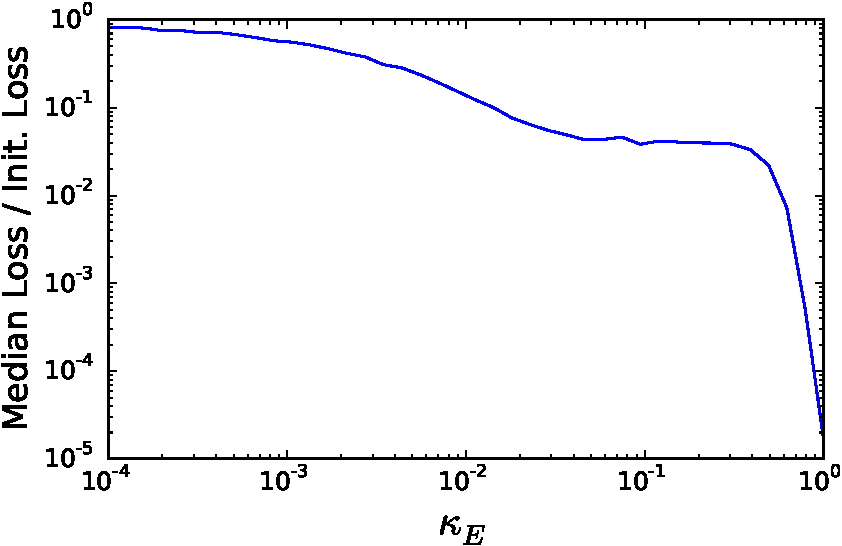
\includegraphics[width=0.75\textwidth]{kappa_E-failure-crop.pdf}
    \end{center}
    \caption{\label{fig:sensitivity-kappa}
        Sensitivity of inversion model \maineq{inv-model} with PGH. The median loss
        over 6,000 trials after 100 measurements is shown as a function of $\kappa_E$.
        For clarity, we normalize the median loss by the initial loss (that is, the median
        loss
        before performing any rejection filtering updates). 
    }
\end{figure}

% NB: not using refs to avoid problems with the split.
Theorem 1 in the main body guarantees a bound on the error in a particular Bayes update due to
$\kappa_E$ being chosen smaller than $\max_x P(E|x)$ for evidence $E$.
However, this only holds for a single update, such that it is not immediately clear
how such errors propagate for an entire \emph{set} of experiments. This is especially
important for heuristic online experiment design, such as via the particle guess heuristic,
or for active learning. To address this, here we show the effects of choosing an inappropriate $\kappa_E$
for the frequency estimation model of \maineq{inv-model}. 

In particular,
we use the particle guess heuristic to design 100 measurements~\cite{wiebe_efficient_2015}, then update using
and 100 rejection filter attempts per measurement, with a recovery factor of
$r=2\%$. We then report in \fig{sensitivity-kappa} the median loss of this procedure as a function
of $\kappa_E$. Importantly, since the this experimental guess heuristic tends to result in likelihoods with
peaks of order unity, any $\kappa_E < 1$ will generate bad samples with high probability over the $m$ particles.

We see that taking $1>\kappa_E\gtrsim 2/3$ does not prevent the algorithm from learning the true model rapidly, although it certainly does
degrade the quadratic loss after $100$ measurements.  On the other hand, as $\kappa_E$ approaches zero the evidence of learning dissapears.  This is to be expected since if $P(E|x)>1$ for all $x$ then all samples are accepted and the approximate posterior will always equal the prior.  We similarly notice evidence for modest learning for $\kappa_E < 0.5$, and note that a plateau appears in the loss ratio for $\kappa_E \in [0.04,0.4]$ where the loss ratio does not monotonically grow with $1/\kappa_E$.  This illustrates that learning still can take place if a value of $\kappa_E$ is used that
is substantially less than the ideal value.  The ability to tolerate small values of $\kappa_E$ is important in cases where $\kappa_E$ is not known apriori and empirical values, such as those obtained via Monte--Carlo sampling, must be used to make the rejection probability polynomially small.



%=============================================================================
\section{Batched Updating}
\label{app:batched-updates}
%=============================================================================

Although we focused in the main body on memory restricted applications, it is also possible to exploit the fact that the
rejection sampling procedure is inherently parallelizable.
This comes at the price of increasing the overall
memory usage. Here, we describe a batched form of our algorithm, assuming a model in which samples are sent by a server to individual processing nodes and the accepted samples are then returned to the server.

\begin{algorithm}
    \caption{Batched update for \CRej}
    \label{alg:batchcrej}
    \begin{algorithmic}
        \Require Prior distribution $\pi:\mathbb{R}^D \mapsto [0,1]$, array of evidence $\vec{E}$, number of attempts $m$, a constant $0<\kappa_E\le 1$, a recovery factor $r \ge 0$, the prior mean $\mu$ and the covariance matrix $\Sigma$.
%        and a mapping $\operatorname{F}$ between $(\mu,\sigma^2)$ to a family of probability distributions that has mean $\mu$ and covariance matrix $\Sigma$. Typically $F$ will yield a Gaussian distribution but other possibilities exist.
        \Ensure  The mean and coviariance matrix of updated distribution $\mu$,$\Sigma$ and $N_a$ which is the number of samples accepted.
        \Function{BatchUpdate}{$\vec{E}$, $m$, $\kappa_E$, $\mu$, $\Sigma$, $r$, $N_{\rm batch}$}
  \State{$(M,S,N_a) \gets 0$}
          \For{{\bf each} $i \in 1 \to N_{\rm batch}$}
  \State Pass $\vec{E},m,\kappa_E, \mu,\Sigma,r$ to processing node $i$.
  \State Set local variables $(\mu^{i}, \Sigma^{i},N_a^{i})\gets \Call{RFUpdate}{\vec{E},m,\kappa_E,\mu,\Sigma,r}$.
  \If{$N_a^i >0$}
  \State $M^i \gets \mu^i N_a^i$
  \State $S^i \gets (N_a^i-1)\Sigma +N_a^i\mu\mu^T$ 
  \State Pass $N_a^i$, $M^i$ and $S^i$ back to the server.       
  \Else \State Pass $(0,0,0)$ back to the server.
  \EndIf
  \EndFor
    \If{$\sum_i N_a^i > 0$}
     \State $\mu\gets \sum_i M^{i}/\sum_i N_a^i $
     \State $\Sigma \gets \frac{1}{\sum_i N_a^i -1}\left(\sum_i S^i - \sum_i N_a^i \mu\mu^T \right)$
  \State\Return $(\mu,\Sigma,N_a)$
   \Else
  \State\Return $(\mu, (1+r)\Sigma),N_a)$

   \EndIf
          
        \EndFunction
    \end{algorithmic}
\end{algorithm}



%=====================================================================
\bibliographystyle{unsrt}
\bibliography{qsmc}
%=====================================================================


\end{document}